%-------------------------------------------------------------------------------
% gettext
%-------------------------------------------------------------------------------
%
% \file        gettext.tex
% \library     Documents
% \author      Chris Ahlstrom
% \date        2024-02-15
% \update      2024-03-22
% \version     $Revision$
% \license     $XPC_GPL_LICENSE$
%
%     Provides a description of the modified gettext.h header file and
%     the gettext module that reimplements parts of it.
%
%-------------------------------------------------------------------------------

\section{GNU Gettext and Its Potext Replacements}
\label{subsec:gettext_code}

   This section briefly covers the public functions and macros of
   \textsl{GNU Gettext} and our replacements for them.
   Here are the main differences:

   \begin{itemize}
      \item All implementations are functions; no macros are used.
      \item All functions are inside the \texttt{po} namespace.
      \item All character pointers are replaced by \texttt{std::string}.
      \item Lookups are done via \texttt{.po} files, at present.
      \item None of the functions with a "category" parameter are
         implemented at this time.
         Those function would seem to need to find an load up another
         \texttt{dictionary} object.
         Also, by far the most common translation files on a \textsl{UNIX}
         system are in the \texttt{LC\_MESSAGE} subdirectories.
   \end{itemize}

\subsection{GNU Gettext Header File}
\label{subsec:gettext_gnu_header_file}

   This section provides a walkthrough of the \texttt{gettext.h} header file
   of the \textsl{Potext} library.
   This is useful in understanding \textsl{Gettext} versus \textsl{Potext}.

   Let us survey the important functions and macros that are used in
   the \texttt{gettext.h} header file
   (see \texttt{/usr/include/libintl.h}):

   \begin{itemize}
      \item \texttt{ENABLE\_NLS}.
         If defined in a GNU automake project, this includes the
         \texttt{libintl.h} header file, which is not needed in
         an application using the \textsl{Potext} library for translation.
         NLS can be disabled via \texttt{--disable-nls}.
      \item \texttt{DEFAULT\_TEXT\_DOMAIN}.
         If \texttt{ENABLE\_NLS} is defined, this macro causes
         \texttt{gettext} to be defined as \texttt{dgettext}, and
         \texttt{ngettext} to be defined as \texttt{dngettext}.
         If \texttt{ENABLE\_NLS} is \textsl{not} defined, then the following
         "functions" are "voided":
         \begin{itemize}
            \item \texttt{gettext}
            \item \texttt{dgettext}
            \item \texttt{dcgettext}
            \item \texttt{ngettext}
            \item \texttt{dngettext}
            \item \texttt{dcngettext}
            \item \texttt{textdomain}
            \item \texttt{bindtextdomain}
            \item \texttt{bind\_textdomain\_codeset}
         \end{itemize}
      \item \texttt{DEFAULT\_TEXT\_DOMAIN} revisited.
         If defined, more macros are defined, for message-context support.
         These call \texttt{pgettext\_aux}
         or \texttt{npgettext\_aux}
         \begin{itemize}
            \item \texttt{pgettext}
            \item \texttt{dpgettext}
            \item \texttt{dcpgettext}
            \item \texttt{npgettext}
            \item \texttt{dnpgettext}
            \item \texttt{dcnpgettext}
         \end{itemize}
      \item \texttt{GNULIB\_defined\_setlocal}.
         If defined, uses the \texttt{rpl\_setlocale} from \textsl{gnulib}
         as \texttt{setlocale}.
      \item \texttt{gettext\_noop}.
         A pseudo function that marks code for extraction of messages, but
         does not call \texttt{gettext}.
      \item \texttt{pgettext\_expr}. Calls \texttt{dcpgettext\_expr()}.
      \item \texttt{dpgettext\_expr}. Calls \texttt{dcnpgettext\_expr()}.
   \end{itemize}

   Do we want \textsl{potext} to be a drop-in replacement for all this stuff?
   We shall try!

\subsection{Gettext Module}
\label{subsec:gettext_module}

   The \texttt{gettext} module provides a reimplementation of
   \textsl{GNU Gettext} "gettext" functions in the \texttt{po}
   namespace.

   Here, we use the term "module" to describe a set of related functions
   that are not members of a class.
   All functions in this module are in the \texttt{po}
   namespace, or are \texttt{static} and internal to the module.

\begin{figure}[H]
   \centering 
   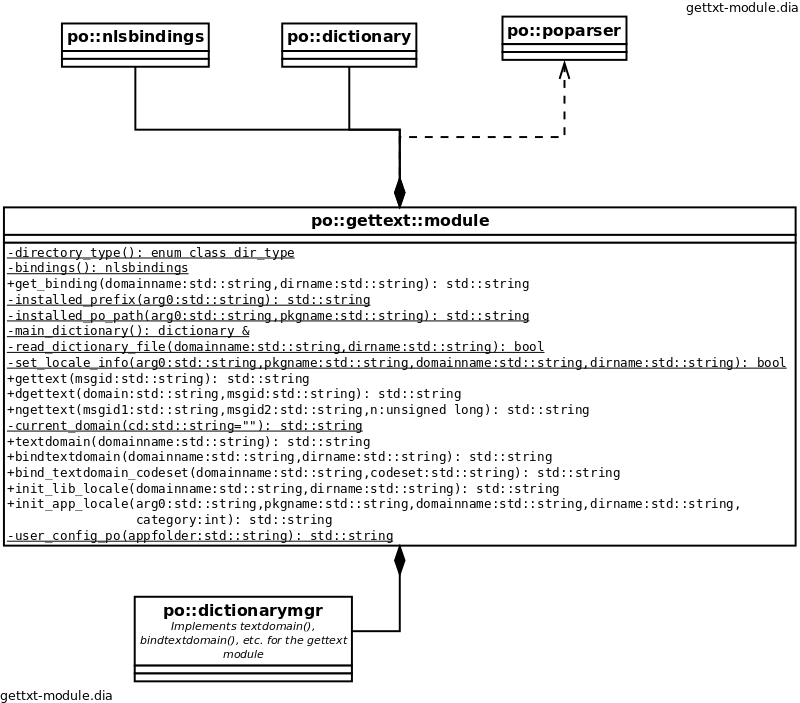
\includegraphics[scale=0.75]{gettext-module.png}
   \caption{Gettext Module (namespace po)}
   \label{fig:gettext_module}
\end{figure}

   We are slowly implement the various "gettext" functions shown in that
   figure, plus some others that are not shown.
   See the next section for a brief discussion of our copy of the
   \texttt{GNU Gettext} header file.

   The following table lists the functions/macros and their purpose and status.
   The implementations are member functions of
   \texttt{po::dictionary} or
   \texttt{po::dictionarymgr} (*); all dictionaries are contained and
   referenced in \texttt{po::dictionarymgr}, either as the main dictionary
   or a dictionary selected based on domain.
   Fall-back functions are noted for some "none" implementations.

   \begin{table}[H]
      \centering
      \caption{Gettext Functions}
      \label{table:potext_gettext_functions}
      \resizebox{\textwidth}{!}{%
      \begin{tabular}{l l p{7cm}}

         \textbf{Function} & \textbf{Implementation} & \textbf{Purpose} \\

         \texttt{textdomain()} & textdomain() * &
            Set or change the current global domain for the
            \texttt{LC\_MESSAGE} category. \\

         \texttt{bindtextdomain()} & bindtextdomain() * &
            Set or change the locale directory for the given domain.
            \texttt{LC\_MESSAGE} category.
            The wide-character \texttt{UTF-16} version for \textsl{Windows}
            is not yet implemented. \\

         \texttt{bind\_textdomain\_codeset()} & partial * &
            Set or change the character-set for the given domain.
            \texttt{LC\_MESSAGE} category. \\

         \texttt{gettext()} & translate() &
            Single message ID translation. \\

         \texttt{dgettext()} & translate() &
            Single message ID translation in a specific domain. \\

         \texttt{dcgettext()} & none: dgettext() &
            Single message ID translation in a specific domain
            and specific language category.
            For all get-text functions with a category parameter,
            there is currently no implementation, just a fall-back
            to the non-category version.\\

         \texttt{ngettext()} & translate\_plural() &
            Message ID translation using a specific singular
            or plural form. \\

         \texttt{dngettext()} & translate\_plural() &
            Message ID translation using a specific singular
            or plural form for a given domain. \\

         \texttt{dcngettext()} & none: translate\_plural()&
            Message ID translation using a specific singular
            or plural form for a given domain and a given locale
            category. \\

         \texttt{pgettext()} & translate\_ctxt() &
            Single message ID translation for a given context (e.g.
            "console" versus "gui". The 'p' stands for 'particular'.\\

         \texttt{dpgettext()} & translate\_ctxt() &
            Single message ID translation for a given context and the
            given domain. \\

         \texttt{dpcgettext()} & none: dpgettext() &
            Single message ID translation for a given context,
            given domain, and category
            other than \texttt{LC\_Messages}. \\

         \texttt{npggettext()} & no &
            Probaby worth doing. \\

         \texttt{dnpggettext()} & no &
            Probaby worth doing. \\

         \texttt{dcnpggettext()} & no &
            Probaby not worth doing. \\

      \end{tabular}}
   \end{table}

%-------------------------------------------------------------------------------
% vim: ts=3 sw=3 et ft=tex
%-------------------------------------------------------------------------------
